\section{Attribute selection}
\subsection{Impact}

\begin{frame}
 \frametitle{Attribute selection}
 \begin{center}
  \alert{Which attribute to select ?}
 \end{center}
 For each project, sort metrics by \emph{Information Gain}:\\
 \vspace{0.2cm}
 \begin{tabular}{ll}
  $InfoGain(A_i)$ = & the number of bits of information obtained\\
   & by knowing the value of attribute $A_i$
 \end{tabular}
 \\
 \vspace{0.4cm}
 Then, in a decreasing order of $InfoGain(A_i)$, compute PD, PF and Bal with the NB+log classifier.
\end{frame}
%discarding a redundant metric could improve performance

\begin{frame}
 \frametitle{Impact of attribute selection}
 \framesubtitle{Linux}
 \begin{center}
  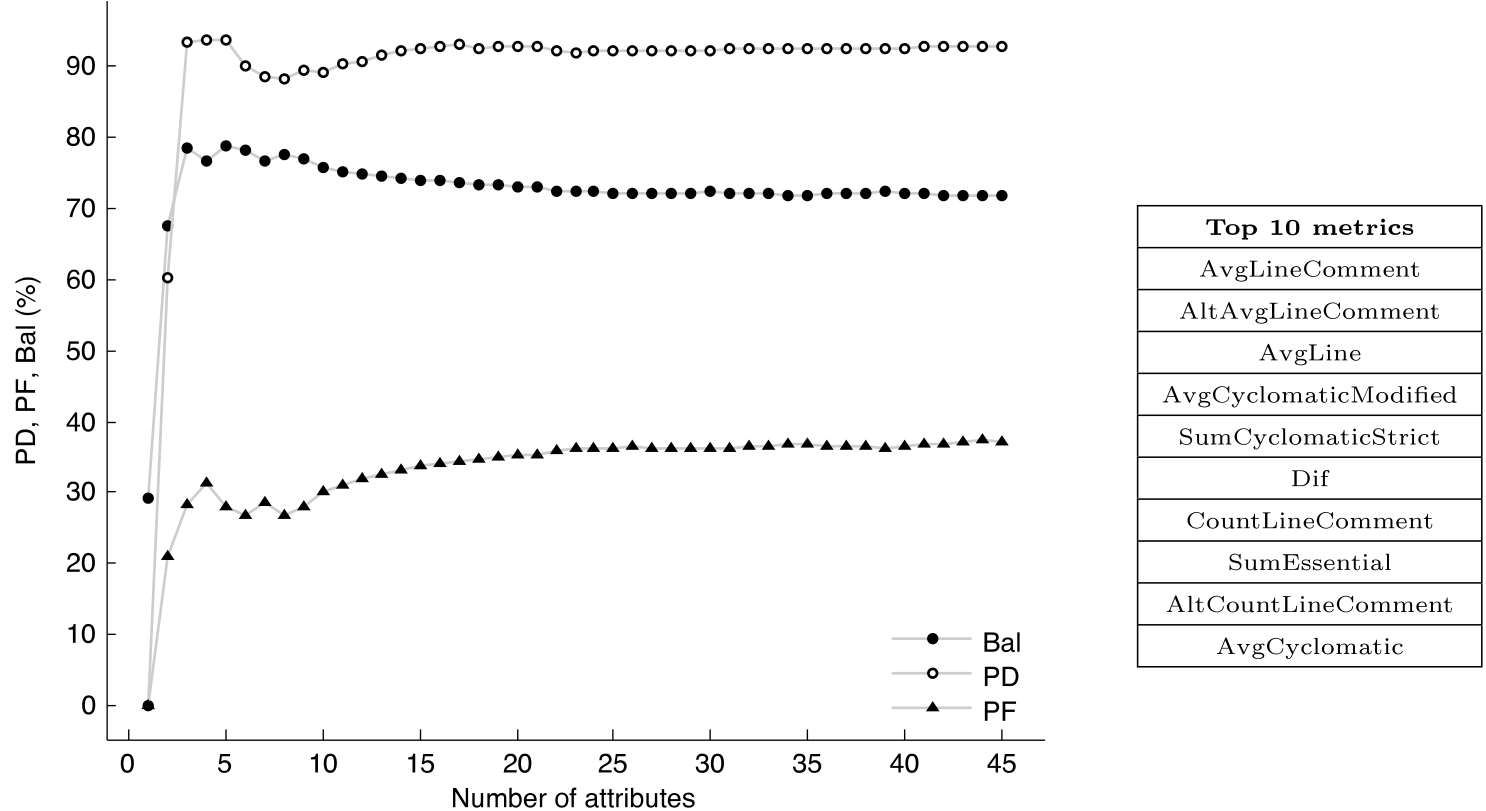
\includegraphics[width=\textwidth]{figures/attributesLinux.png}
 \end{center}
\end{frame}

\begin{frame}
 \frametitle{Impact of attribute selection}
 \framesubtitle{MySQL}
 \begin{center}
  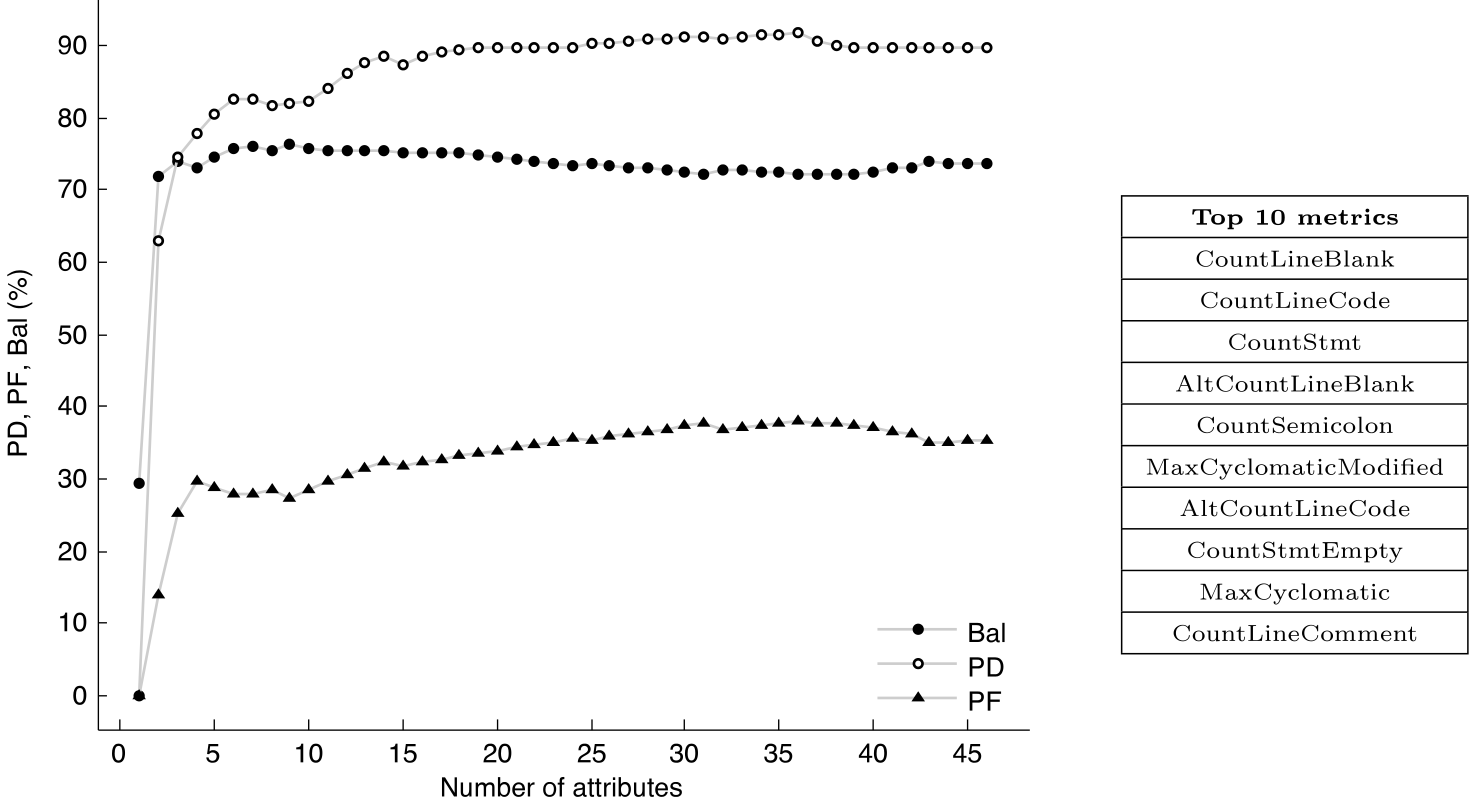
\includegraphics[width=\textwidth]{figures/attributesMysql.png}
 \end{center}
\end{frame}

\begin{frame}
 \frametitle{Impact of attribute selection}
 \framesubtitle{CARDAMOM}
 \begin{center}
  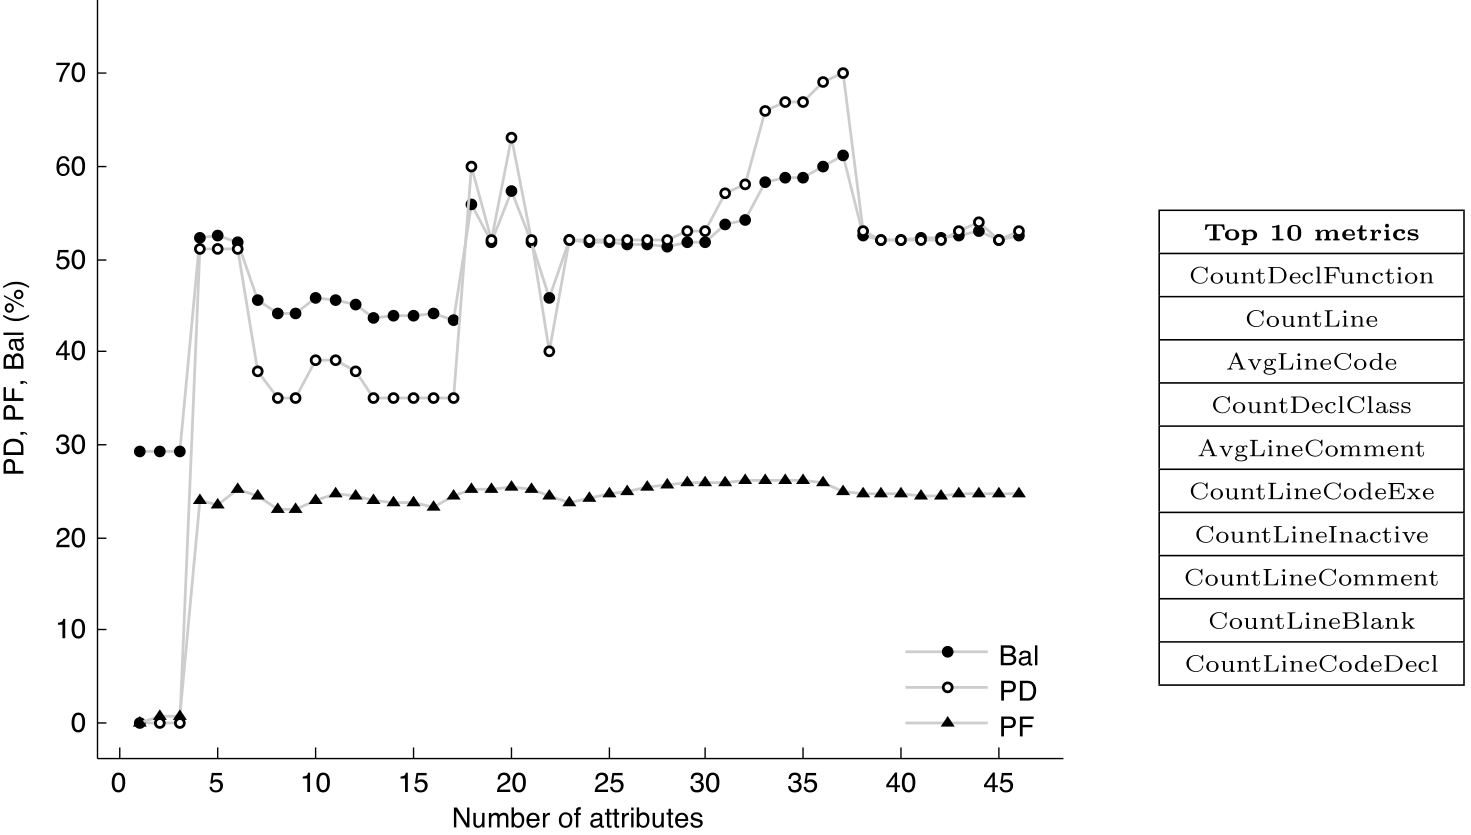
\includegraphics[width=\textwidth]{figures/attributesCardamom.png}
 \end{center}
\end{frame}

\begin{frame}
 \frametitle{Impact of attribute selection}
 \begin{itemize}
  \item Top metrics not the same
  \item Need about 5 top metrics
  \item With all metrics, nearly the same results than with 5
 \end{itemize}
 \vspace{0.5cm}
 \begin{center}
  $\Longrightarrow$ \alert{We keep the full set of metrics.}
 \end{center}
\end{frame}